Ein Laser besteht aus einem Lasermedium, einer Pumpe und einem Resonator.
Durch Hohspannung wird dem Lasermedium die Pumpenergie zugeführt, welche bewirkt, dass das Lasermedium in einen angeregten Zustand übergeht.
Durch das Einstrahlen von Licht in der passenden Wellenlänge kommt es zur induzierten Emission wie in Abbildung \ref{fig:absemi} zusehen.
Das angeregte Atom fällt auf sein Grundzustand zurück.
Die freiwerdende Energie wird dabei in Form von Photonen ausgesendet, die der einfallenden Strahlung in Energie, Phase und Ausbreitungsrichtung gleicht.
Das einfallende Licht wird auf diese Weise verstärkt.
\FloatBarrier
\begin{figure}
  \centering
  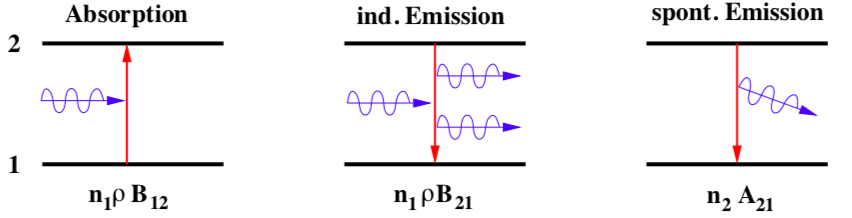
\includegraphics[width=10cm]{absorption.PNG}
  \caption{Absorption und Emission}
  \label{fig:absemi}
\end{figure}
\FloatBarrier
Der Resonator besteht aus zwei Spiegeln, wie in Abbildung \ref{fig:resonator} zu erkennen,  wobei einer dieser Spiegel halb durchlässig ist um ein Teil des Lichtest auszukoppeln.
Die Spiegel werfen das austretende Laserlicht zurück in das Lasermedium.
Auf diese Weise wird der Weg des Lichtes im Lasermedium verlängert und es entsteht ein selbsterregnder Oszilator.
\FloatBarrier
\begin{figure}
  \centering
  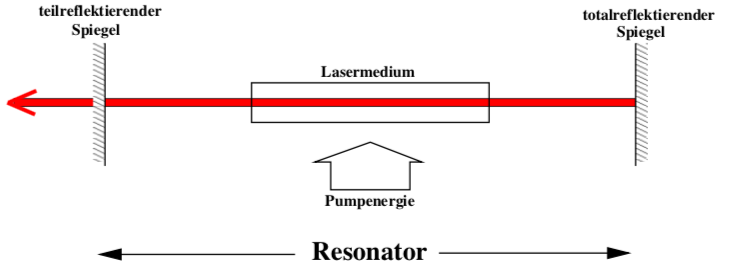
\includegraphics[width=15cm]{resonator.PNG}
  \caption{Aufbau eines Resonators}
  \label{fig:resonator}
\end{figure}
\FloatBarrier
Für eine verstärkung des Lichtstrahls müssen die Resonatorspiegel möglichst Verlustfrei sein.
Die geringsten Verluste erziehlt man mit einem konvokalen Resonator bei dem die Spiegelbrennpunkte an der selben Stelle liegen.
Für einen optisch stabilen Resonator müssen die Verluste geringer sein als die Verstärkung.
Dieser selbsterregende Oszillator erfüllt dann die Bedingung:
\begin{align*}
  0\leq g_1\cdot g_2 <1.
\end{align*}
Der resonatorparameter g ist gegeben durch:
\begin{align*}
  g_i=1-\frac{L}{r_i}
\end{align*}
wobei r den Krümungsradius der Spiegel und L die Resonatorlänge darstelt.
Der Krümungsradius hat Einfluss auf die Sabilität des Resonartors.

Die Resonanzbedingung für stehende Wellen ist, da die Resonatorlänge L viel größer ist als die Wellenlänge $\lambda$, für viele Frequenzen erfüllt.
Im Resonator kann es zur Ausbildung von transversalen und longitudinalen Moden kommen wobei eine Mode die Anzahl q der Wellenlängen im Resonator beschreibt.
Niedrige Moden mit hoher Symetrie haben geringere Verluste als größere Moden.
Das hat zurfolge, dass im Resonator nur wenige transversale Moden $l$ und $p$ verstärkt werden.
Das Laguerre-Polynom $L_p^q(u)$ kann den transversalen Modenzahlen $l$ und $p$ zugeordnet werden.
Diese Feldverteilungen der transversalen Moden lassenen sich für einen konvokalen Resonator mit gekrümten Spiegeln beschreiben durch:

\begin{align}
  E_{lpq} &\propto \cos(l \varphi)\frac{(2\rho)^2}{(1+Z^2)^{\frac{(1+l)}{2}}}
  L_p^q\left(\frac{(2\rho)^2}{1+Z^2}\right)\cdot exp \left(-\frac{\rho^2}{1+Z^2}\right)\\
  &\times exp \left(-i\left(\frac{(1+Z)\pi R}{\lambda}+\frac{\rho^2Z}{1+Z^2}-(l+2p+1)\left(\frac{\pi}{2}-
  \arctan\left(\frac{1-Z}{1+Z}\right)\right)\right)\right)
\label{eqn.feld}
\end{align}
$\rho$ und $Z$ sind dabei gegeben als:
\begin{align*}
  \rho=\left(\frac{2\pi}{R\lambda}\right)^{(\frac{1}{2})}\\
  Z=\left(\frac{2}{R}\right)\cdot z
\end{align*}
Mithilfen von \ref{eqn.feld} kann die Intensitätsverteilung berechnet werden.
Die Mode mit geringstem Verlust ist dei TEM$_{00}$ Mode, da diese keine Nulstellen in transversaler richting aufweist.
TEM$_{lpq}$ steht dabei für transverse electromagnetic mode.
Der Laserstrahl besitzet eine gaußverteilte Intensitätskurve.
In der Strahlmitte ist die Intensität am größten und nillmt zu den Rändern hin ab.
Die Intensitätsverteilung ist gegeben als:
\begin{align*}
  I(r)=I_0e^{\frac{-2r^2}{\omega ^2}}
\end{align*}
$I_0$ beschreibt dabei die maximale Intensitär.
Der Abstand zur optischen Achse  wird mit $r$ abgekürzt.
Der Strahlradiuns $\omega$ kann zudem in abhängigkeit vom Abstand $Z$ zur minimalen Strahltallie $\omega_0$ angegeben werden.
\begin{align*}
  \omega(Z)=\omega_0\sqrt{1+\left(\frac{\theta_Z}{\omega_0}\right)^2}
\end{align*}
$\theta$ beschreibt dabei die Strahldivergenz des Guaßschen Strahls.
\begin{align*}
  \theta=\left(\frac{\lambda}{\pi}\right)\omega_0
\end{align*}
